\section{Related Work}

% Various approaches for document image classification have been proposed over the years. Generally, document image classification approaches are divided into two major groups, structure/layout based, and content based. This section provides an overview of some important works which have been reported in reference to structure or content based document classification.% \subsection{Content based Document Classification}

Over the years, different methods have been proposed for document image classification. The overall classification methods can be divided into three distinct categories.
The first category exploits structure and layout similarities, while the second focuses on developing local and global features that could be used for document classification. The third category is based on deep \ac{cnn}s that extract the features automatically for document classification. This section provides a summary of the important related work regarding the above mentioned three categories.

\begin{figure*}
    \begin{subfigure}{0.22\linewidth}
        \centering
        \fbox{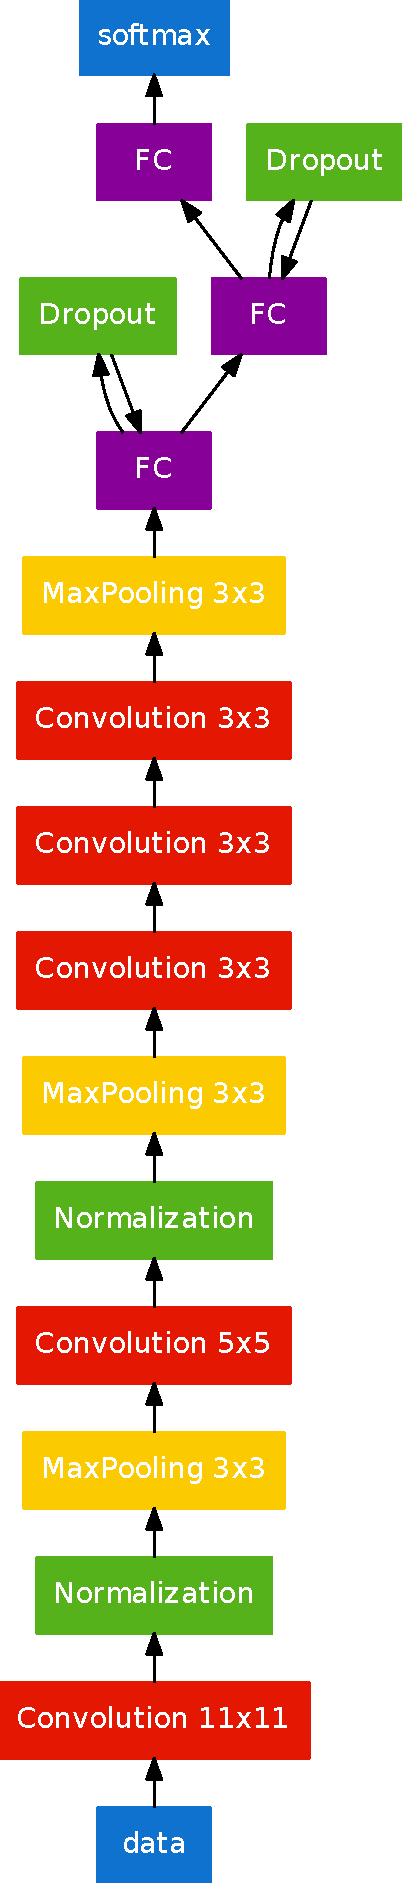
\includegraphics[height=0.65\textheight]{architectures/alexnet.pdf}}
        \subcaption{AlexNet}
        \label{fig:alexnet}
    \end{subfigure}
    \begin{subfigure}{0.21\linewidth}
        \centering
        \fbox{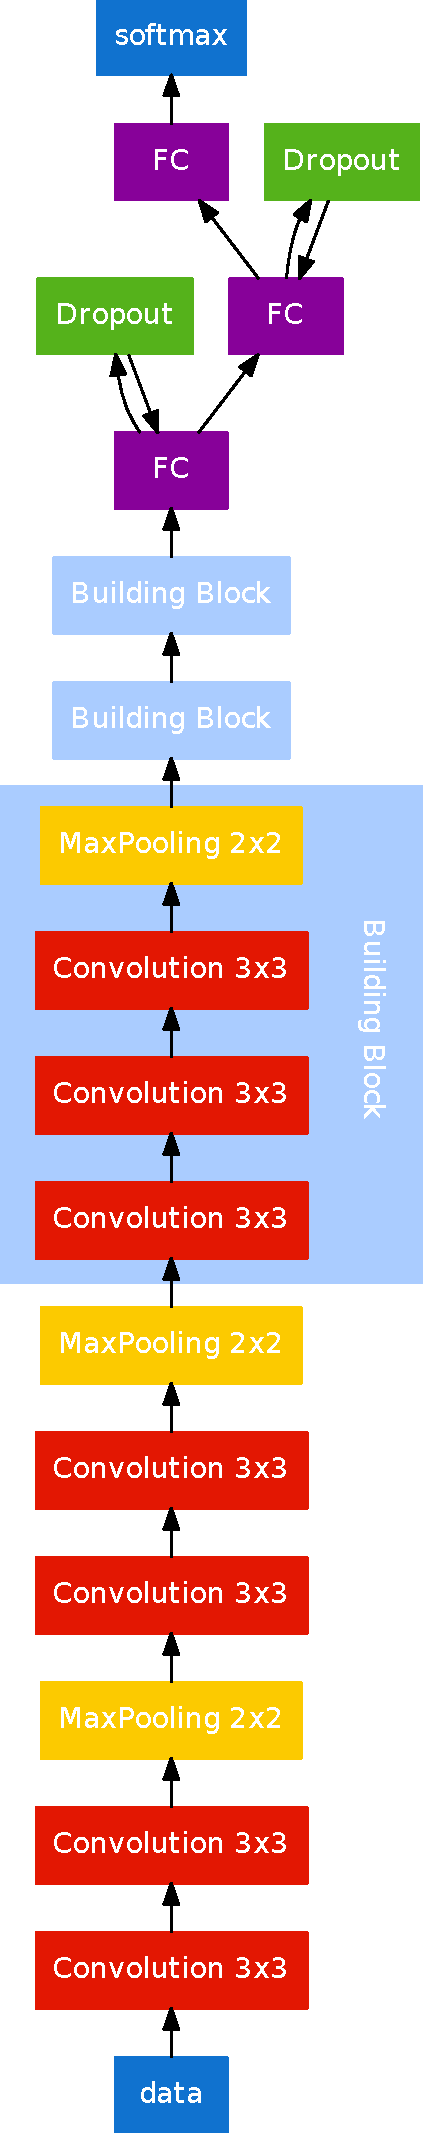
\includegraphics[height=0.65\textheight]{architectures/vgg.pdf}}
        \subcaption{VGG-16}
        \label{fig:vgg}
    \end{subfigure}
    \begin{subfigure}{0.36\linewidth}
        \centering
        \fbox{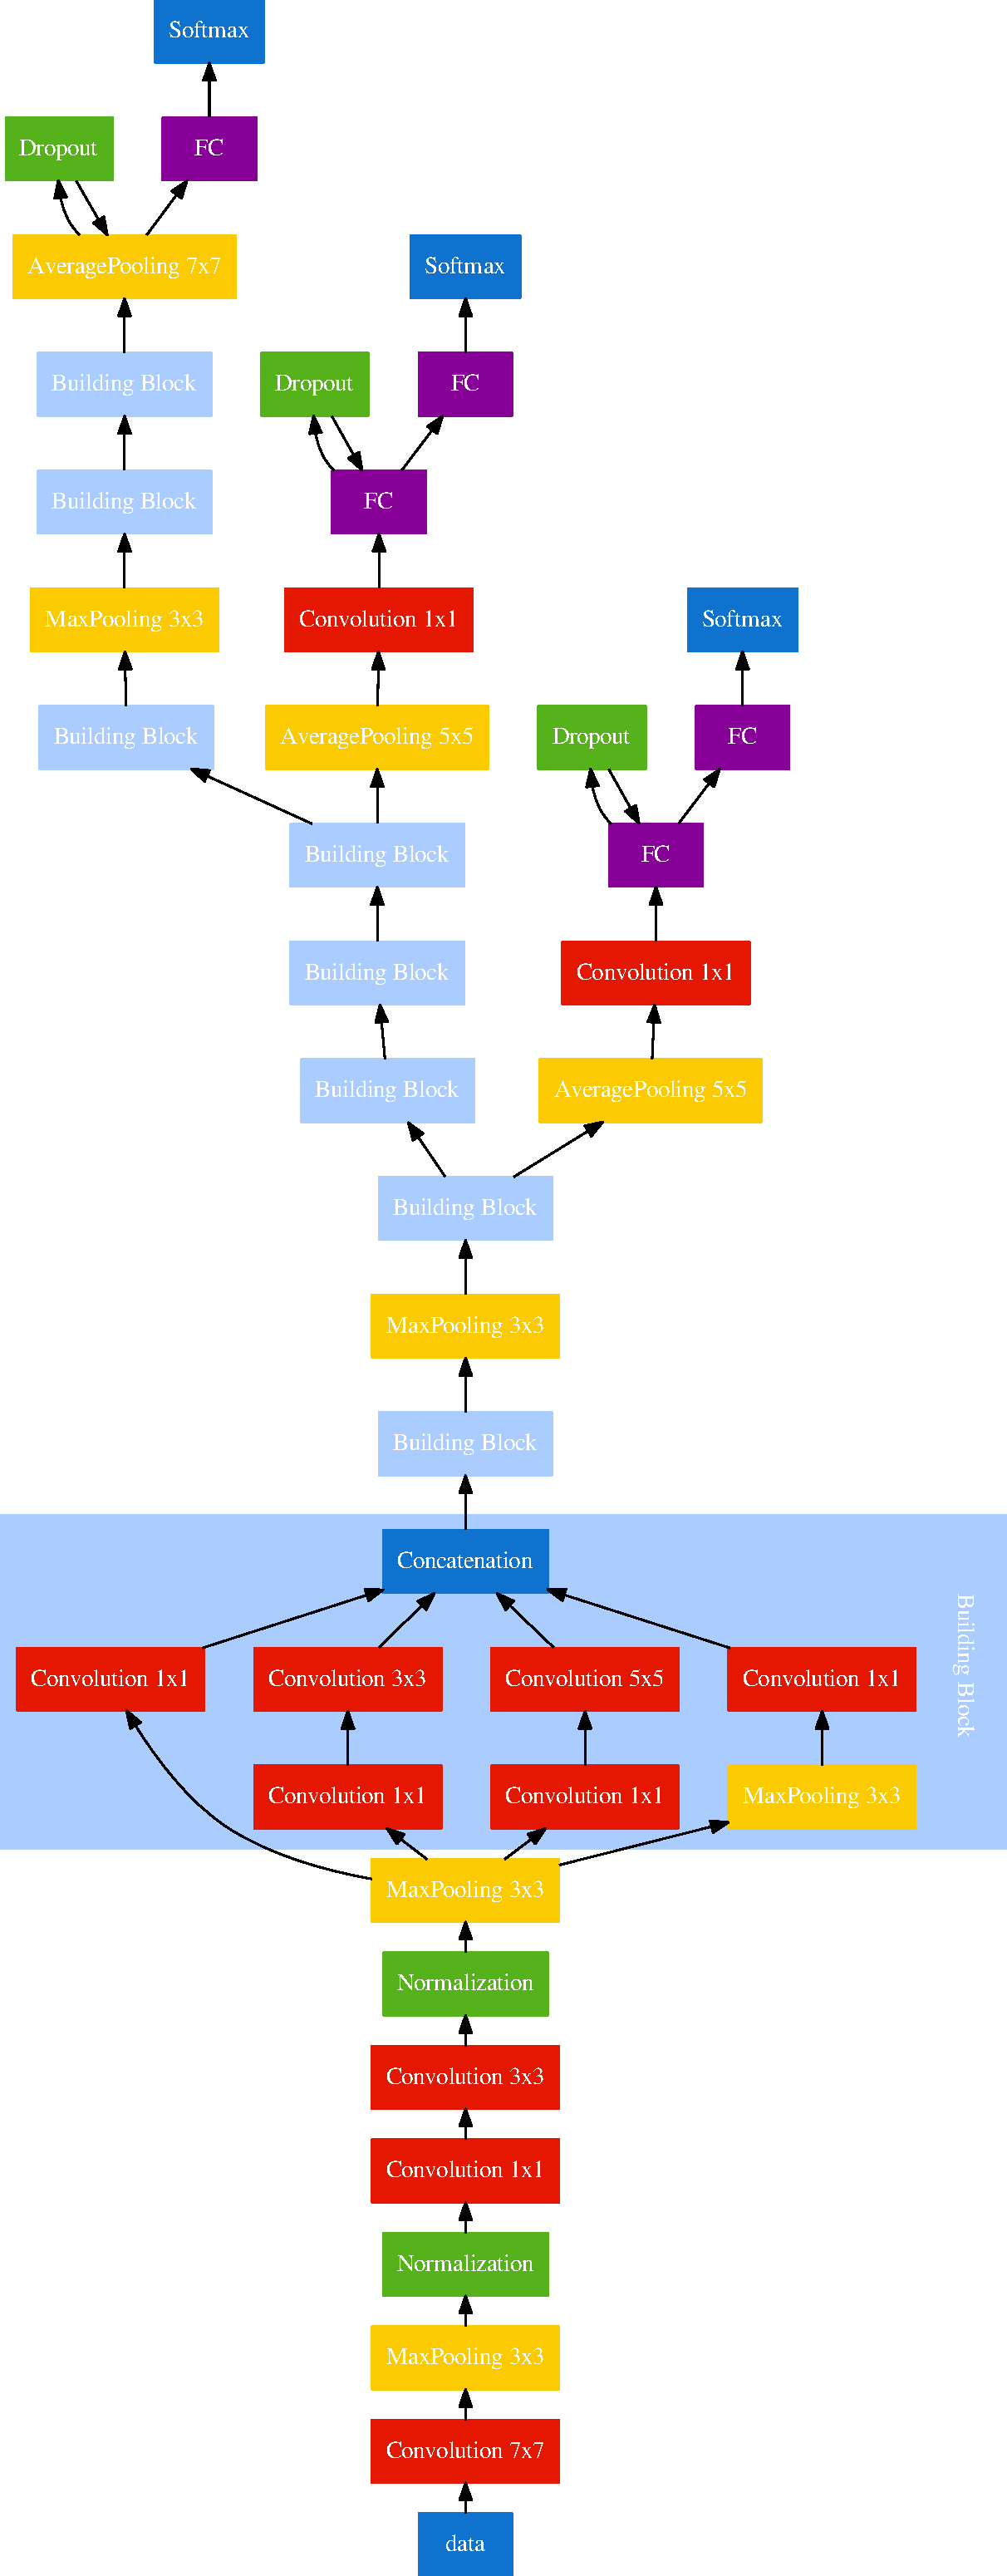
\includegraphics[height=0.65\textheight]{architectures/googlenet.pdf}}
        \subcaption{GoogLeNet}
        \label{fig:googlenet}
    \end{subfigure}
    \begin{subfigure}{0.19\linewidth}
        \centering
        \fbox{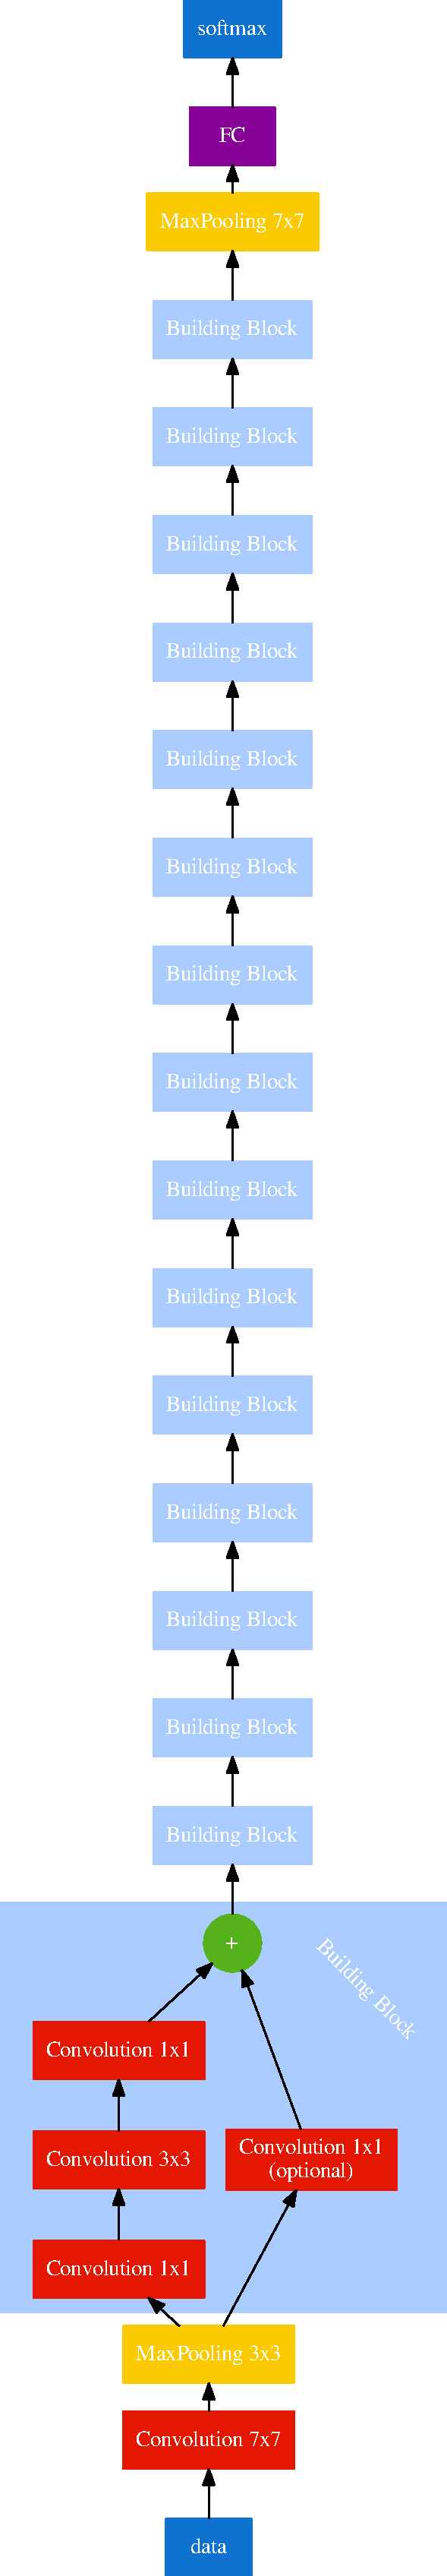
\includegraphics[height=0.65\textheight]{architectures/resnet.pdf}}
        \subcaption{ResNet-50}
        \label{fig:resnet}
    \end{subfigure}
    \caption{Deep CNN architectures used in this work}
    \label{fig:deepcnn}
\end{figure*}

Dengel and Dubiel~\cite{doclass_Dengel95} used layout structure printed documents. They used top-down induction in decision trees to convert printed documents into a complementary logical structure.
Bagdanov and Worring~\cite{doclass_Bagdanov2001} classify machine-printed documents by using the Attributed Relational Graphs (ARGs).
Byun and Lee~\cite{doclass_Byun2000} used parts of the documents for the recognition. They reasoned that processing complete documents is time-consuming. The document classification was performed on parts of the documents using DP algorithm. Their approach was fast but the applicability is limited to forms. Shin and Doermann~\cite{doclass_shin} proposed an approach that used layout structural similarity for full or partial image matching for retrieval. 
Kevyn and Nickolov~\cite{Collins-thompson02aclustering-based} used both the layout and the text features for matching the documents for retrieval. 

Jayant et al.~\cite{doclass_Kumar12} propose a method that relies on the patch code words derived from the document images. The code book is learned independently of the class labels of the documents. In the first step, the images are recursively partitioned both in horizontal and vertical direction for modeling spatial relationships. Subsequently, a histogram for each partition is calculated that is used for the classification.
Following the same idea of developing the code book, another work presented by Jayant et al.~\cite{doclass_Kumar14} build a codebook of SURF descriptors extracted from training images. Then, histograms of codewords are created similar to~\cite{doclass_Kumar12}. A Random Forest classifier is used for classification. The applicability of the approach is shown in the presence of limited data.
Chen et al.~\cite{doclass_Chen12} propose a method based on low-level image features to classify documents. The approach is limited to structured documents. An important point is that one could obtain the registration of two images by matching the feature points.
Joutel et al.~\cite{doclass_Joutel2007} proposed a method that used curvelet transformation for indexing and querying the documents at different image scales. Their method is designed particularly for large databases of handwritten manuscripts. Kochi and Saitoh~\cite{doclass_Kochi99} used textual descriptions of document images for information extraction from documents. The method is limited to semi-structured documents and assumes a pre-defined knowledge is available for the document classes.
Reddy and Govindaraju~\cite{doclass_umamaheswara08} used binary images for the classification of the documents. They use pixel information and calculate pixel densities.  They used k-means clustering supported by adaptive boosting. The method is evaluated on the benchmark NIST scanned special tax form databases $2$ and $6$.

%The approach only deals with structured documents which are mostly-text and with pre-printed contents.  doclass_Kumar12,doclass_Chen12, doclass_Kumar14

% Jayant et al.~\cite{doclass_Kumar12} propose a method based on statistics of patch code words. Starting with a set of wanted and a random set of unwanted images, raw-image patches extracted from the unlabeled images to learn a code book. Spatial relationships between patches are modelled by recursively partitioning the image horizontally and vertically and a histogram of patch-codewords is computed for each partition. 

% In another work, Jayant et al.~\cite{doclass_Kumar14} build a codebook of SURF descriptors extracted from some training images. Then histograms of codewords are created similar to~\cite{doclass_Kumar12}. Later a Random Forest classifier is used for classification. The system performs reasonably even for limited training data. Chen et al.~\cite{doclass_Chen12} propose a method based on SIFT descriptors to classify documents. The approach only deals with structured documents which are mostly-text and with pre-printed contents.


%low level pixel density information from the binary images. The proposed system is based on the k-means algorithm and supported by adaptive boosting. The results are reported on the benchmark NIST scanned special tax form databases $2$ and $6$.


% Joutel et al.~\cite{doclass_Joutel2007} use Curvelet transform as a multiscale method for indexing linear singularities and curved handwritten shapes in documents images. 
% Their method detects oriented and curved fragments at different scales and searches for similar handwritten samples in large manuscripts databases. 
% Kochi and Saitoh~\cite{doclass_Kochi99} compare  the textual elements of document images. The presented system is robust against shifts or noise in the target documents and can handle semi-formatted documents..
% Reddy and Govindaraju~\cite{doclass_umamaheswara08} use low level pixel density information from the binary images. The proposed system is based on the k-means algorithm and supported by adaptive boosting. The results are reported on the benchmark NIST scanned special tax form databases $2$ and $6$.
% \subsection{Structure based Document Classification}



%Based on Layout Structural Similarity doclass_Byun2000, doclass_shin, Collins-thompson02aclustering-based


The pioneering work that performed document classification using \ac{cnn}s used a rather shallow network for classification~\cite{lekang_14_a}. Nevertheless, the proposed approach outperformed structural similarity based methods and shows the potential of automatic feature learning for document classification using \ac{cnn}s. The reason may be that deep networks require a lot of data for training and at that time the standard challenging dataset consisted of only $3,482$ images.
Afzal et. al.~\cite{afzal2015deepdocclassifier} and Harley et. al.~\cite{harley2015evaluation} provided a breakthrough when they showed that it is possible to use transfer learning and the features that are learned from general (daily life) images can be used for the classification of document images~\cite{afzal2015deepdocclassifier}. They achieved a significant improvement over \ac{cnn} based methods that were the \sota at that time.
%Another significant contribution is presented by Harley et. al.~\cite{harley2015evaluation}. 
%The concept of their work was the same as Afzal et. al., however, they used the features from deep \ac{cnn} for document retrieval and showed that validity of their approach.
Another notable contribution by Harley et. al.~\cite{harley2015evaluation} was that they introduced a dataset consisting of $400,000$ documents divided into $16$ classes.
This allowed for the evaluation of deep neural networks using a significant amount of data. 

The \sota in deep \ac{cnn}s has advanced significantly in recent years and there has been no comprehensive study regarding the impact of deep architectures for document classification. Moreover, there is no study that explores transfer learning from document images and also there is no report of the impact of the amount of training images. The presented work takes into account these issues and performs a comprehensive set of experiments to fill the gaps that exist. Eventually, this study leads to an approach that can reduce the error by more than half and therefore provides another leap forward in the domain of document image classification.


% Deep convolutional networks have shown successful results on large benchmark datasets consisting of more than one million images, such as ImageNet~\cite{cnn_alexnet_nips2014}.
% Alex et al.~\cite{cnn_alexnet_nips2014} trained a large, deep convolutional neural network to classify the $1.2$ million high-resolution images in the ImageNet LSVRC-2010 contest into $1000$ different classes. An important finding was that the learned deep representation is transferable across different tasks.
% Sermanet et al.~\cite{conf/cvpr/SermanetKCL13} suggested to use unsupervised pre-training, followed by supervised fine-tuning for pedestrian detection. Similarly, supervised pre-training was proved helpful in different computer vision and multimedia settings w.r.t. a concept-bank paradigm~\cite{TorresaniSzummerFitzgibbon10}. Recently, Girshick et al.~\cite{journals/corr/GirshickDDM13} showed that, for dealing with scarce data, supervised pre-training on larger data and then fine-tuning on smaller problem-specific dataset improves classification results. Based on this background, to the best of our knowledge, this paper is the first attempt ever when pre-trained CNN are optimized for document image classification.

